% Provenance (never printed): see sources/outline_sources.md (Year 2: field and laboratory methods ---
% igneous and metamorphic petrography, chemical analysis by XRF, ICP-MS and microprobe, isotope mass
% spectrometry, a mapping campaign). Modelled on Book 3 ch. 6.
% Textures: BGS RR 99-02 (Robertson 1999), Open University Virtual Microscope, Carleton BH250,
% UCSB Geology 102C (Hacker); QAPF: BGS RR 99-06 (Gillespie and Styles 1999); instruments: SERC
% Geochemical Instrumentation and Analysis sheets (EPMA, WDS, XRF, TIMS, MC-ICPMS); XRF procedure
% and reference-material results: USGS OFR 02-223 and its chapter T (Taggart and Siems 2002); Sr
% isotopes: CIAAW; spike and mass bias: Cheong, Jeong and Kwon (2014). Ledger rows in
% sources/ledger/book4.md; curves and stations from figdata/bachelor-2/labmethods.py, numbers from
% the Book 4 second-writer scratch calculator calc/ch31.py. Observation only: the professional work
% is described in the third person.
\chapter{野外与实验方法 II}\label{ch:b2:field-lab-methods-2}

本书岩石学各章中的每一个数，最初都是袋中的一块岩石、显微镜下的一张薄片，
以及仪器中的一份粉末。投在相图上的矿物成分，决定熔岩命名的二氧化硅含量，
追踪地幔源区的锶同位素比值，
都出自一连串操作；这些操作始于露头，每一个环节都带有误差。
本章沿着这一链条，考察瓦尔登丘陵基底的岩石：先读取薄片中的结构，
再统计矿物含量，继而分析全岩，随后分析单矿物，最后分析同位素，
并在每一步追问结果的可靠程度。

\begin{recall}
\textbf{来自第 1 册}：野外观测点、野外记录簿、定向样品、
薄片、偏光显微镜、单偏光、正交偏光；造岩矿物的光学鉴定；
由氧化物分析在固定氧原子数下换算矿物化学式，
并由电荷平衡求三价铁；面理与片理；等时线、初始比值与最小二乘直线。
\textbf{来自化学分册}：质谱法、电感耦合等离子体；标准曲线、
检出限、定量限、精密度、正确度、偏差、重复性、平均值的标准差。
\textbf{来自物理分册}：特征 X 射线与莫塞莱定律；布拉格定律；
表面张力；不确定度的传播。
\textbf{来自数学分册}：二项分布及其均值与方差。
\textbf{来自\cref{ch:b2:magmatic-series}}：\omterm{def:b2:magmatic-series:qapf}{实际矿物组成}，\omterm{def:b2:magmatic-series:qapf}{QAPF 图解}。
\textbf{来自\cref{ch:b2:isotope-geochemistry}}：\omterm{def:b2:isotope-geochemistry:tracer}{放射成因同位素示踪剂}，\omterm{def:b2:isotope-geochemistry:standards}{同位素参考标准}。
\end{recall}

\section{岩石学：作为历史的结构}\label{sec:b2:field-lab-methods-2:petrography}

第 1 册用偏光显微镜鉴定矿物。岩石学家还要读取颗粒的排列方式，
因为排列记录了颗粒生长的先后次序。两种结构是
熔体结晶的最常见见证，以及
固态重结晶的最常见见证。

\begin{definition}[辉绿结构，粒状变晶结构]\label{def:b2:field-lab-methods-2:textures}
当大颗粒辉石包裹着取向随机的小斜长石板条时，火成岩具有\emph{辉绿结构}\index{辉绿结构}；
该结构典型见于辉绿岩、辉长岩和玄武岩。
变质岩具有\emph{粒状变晶结构}\index{粒状变晶结构}，指其为大小大致相同、近似等轴晶体的集合体，
多数晶体为他形，
其直边在三联点处以接近 \ang{120} 的角相交。
\end{definition}
% ledger: carletonB:ophitic, ouVM:textures, bgsM:textures

在\omterm{def:b2:field-lab-methods-2:textures}{辉绿结构}的岩石中，被包裹的板条完整、自形，辉石充填其间的空隙：
斜长石先结晶，辉石围绕其生长。\omterm{def:b2:field-lab-methods-2:textures}{粒状变晶结构}中的 \ang{120} 角，
是颗粒有足够时间调整边界的结果；岩石学教学材料把这类三联点视为
化学与结构平衡的标志。该角度由力的平衡决定，晶界沿其公共线拉扯，
犹如肥皂膜（表面张力，来自物理分册）。
% ledger: ouVM:equilibrium

\begin{proposition}[三联点处的角]\label{prop:b2:field-lab-methods-2:triple}
设三条晶界沿一条线相交，其张力（单位面积的能量）分别为 $\gamma_1$，
$\gamma_2$、$\gamma_3$，并设 $\theta_i$ 为除晶界 $i$ 之外的两条晶界之间的夹角。
平衡时，
\begin{equation}
\frac{\gamma_1}{\sin\theta_1} = \frac{\gamma_2}{\sin\theta_2} = \frac{\gamma_3}{\sin\theta_3},
\label{eq:b2:field-lab-methods-2:lami}
\end{equation}
且三个相等的张力相交成三个 \ang{120} 角。
\end{proposition}

\begin{proof}
在垂直于交线的平面内，每条晶界沿其自身迹线以单位长度的力 $\gamma_i$ 拉扯交点。
平衡时三力之和为零，因此首尾相接可构成一个三角形。
三角形中与边 $\gamma_i$ 相对的角为 $\pi - \theta_i$，
其正弦为 $\sin\theta_i$，由三角形的正弦定理即得\eqref{eq:b2:field-lab-methods-2:lami}。
若三个张力相等，则三角形为正三角形，
每个外角 $\theta_i$ 为 $\pi - \pi/3 = 2\pi/3$，即 \ang{120}。
\end{proof}

\begin{omfigure}
\centering
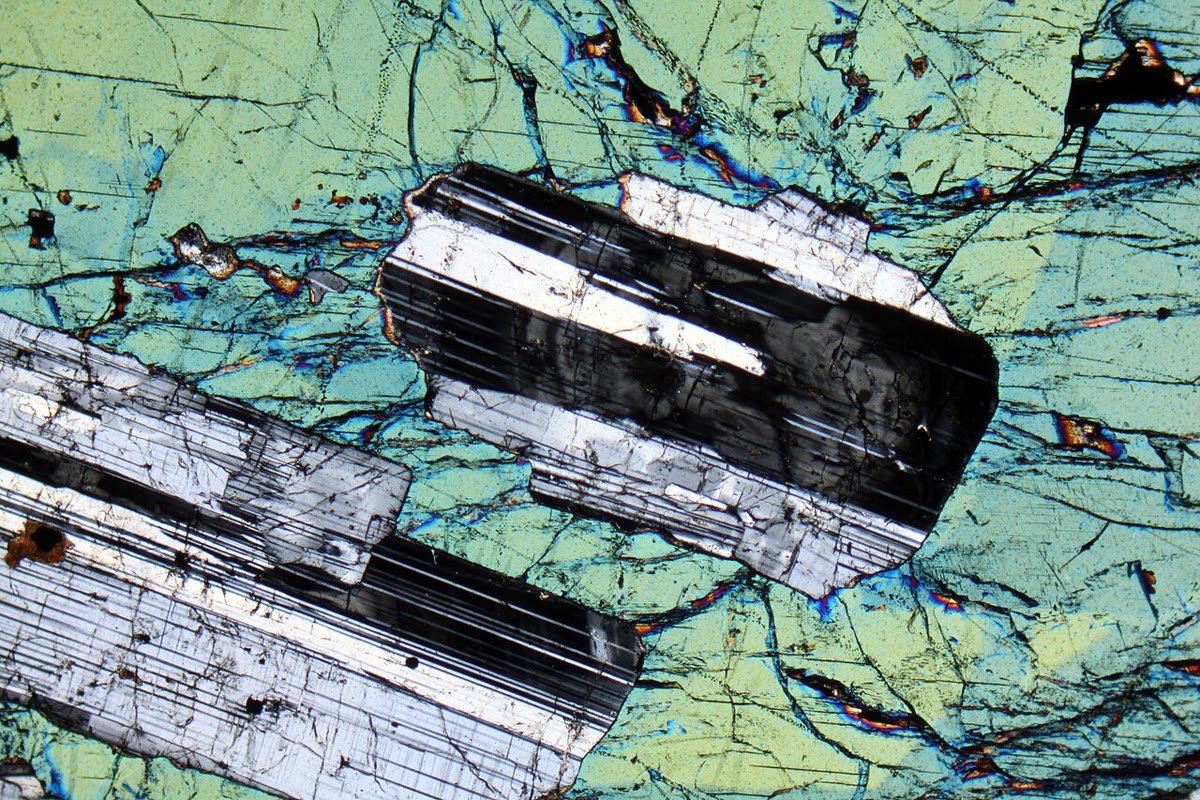
\includegraphics[height=4.6cm]{images/book4/b2-31-ophitic.jpg}\quad
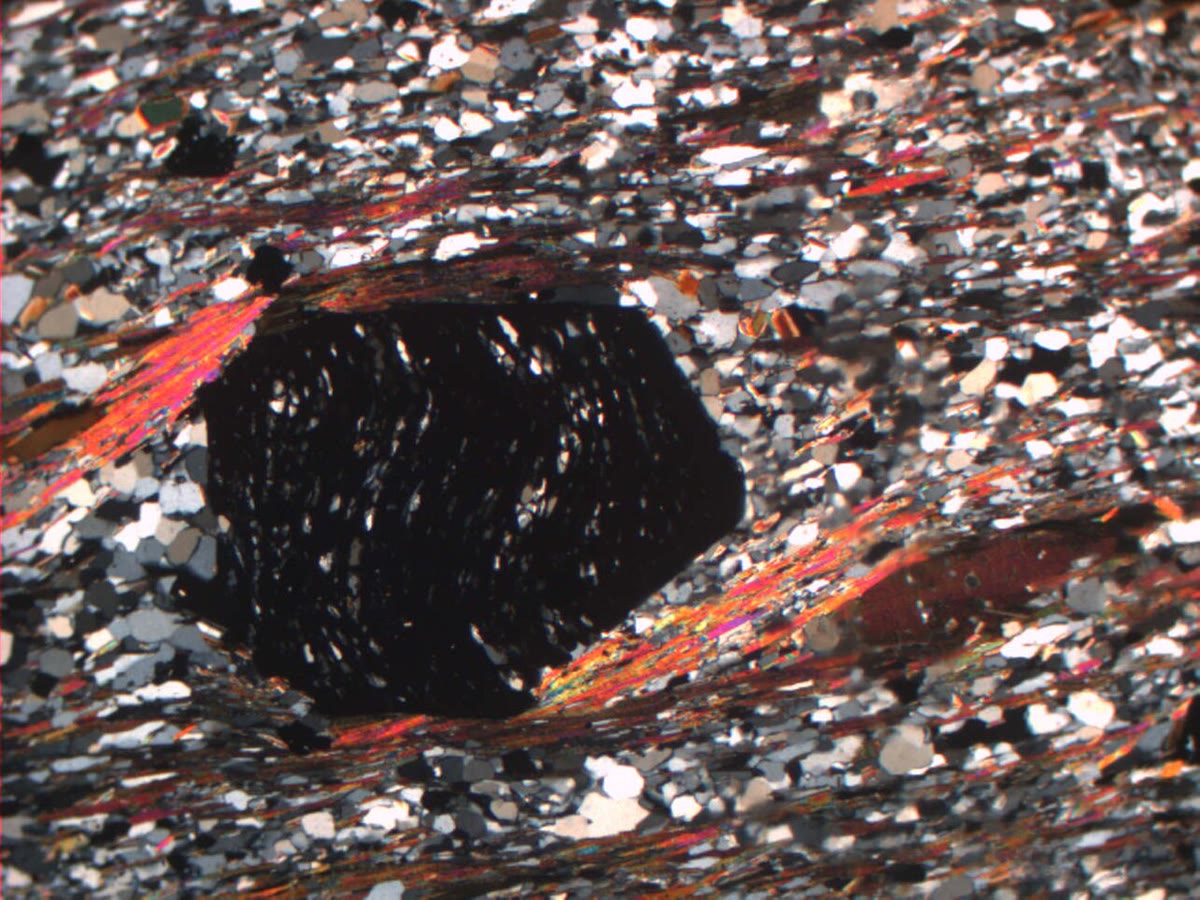
\includegraphics[height=4.6cm]{images/book4/b2-31-garnet-porphyroblast.jpg}
\par\smallskip{\small 正交偏光下的两种结构。左：一颗辉石（蓝色与绿色）单晶，
包裹着因双晶而呈条纹的斜长石板条，即\omterm{def:b2:field-lab-methods-2:textures}{辉绿结构}的排列方式；
视场宽 \qty{7}{mm}。照片：Strekeisen，CC BY-SA 4.0（维基共享资源）。
右：石榴子石–云母片岩。石榴子石因属均质体而呈黑色，是在固态中生长的大晶体；
石英包裹体成串穿过晶体，白云母（亮色）、
黑云母（褐色）与石英（灰色）组成的面理绕其弯曲。照片：Jackdann88，
CC BY 3.0（维基共享资源）。}
\end{omfigure}
% ledger: photo:b2-31-ophitic, photo:b2-31-garnet

变质矿物并非都以相同速度生长。有些矿物会优先长大，形成很大的晶体，
在生长过程中吞没周围的小颗粒。

\begin{definition}[变斑晶，包含变晶，包裹体迹线，反应边]\label{def:b2:field-lab-methods-2:porphyroblast}
\emph{变斑晶}\index{变斑晶}是在\omterm{def:b2:metamorphic-facies:metamorphism}{变质作用}中于较细粒基质内生长的大晶体；
石榴子石、十字石、堇青石和硬绿泥石等可形成变斑晶，
其直径从毫米到数厘米不等。\emph{包含变晶}\index{包含变晶}是
含有许多其他矿物包裹体的变斑晶。\emph{包裹体
迹线}\index{包裹体迹线}是变斑晶内部排列成线的一串包裹体，
它保存了晶体包覆基质时基质的组构。
\emph{反应边}\index{反应边（反应结构）}是完全包围一个正在分解的矿物的一圈或多圈新矿物，
该矿物因与邻近矿物不再稳定而分解，
这是在反应完成之前即被冻结下来的反应结构。
\end{definition}
% ledger: bgsM:textures, ouVM:textures

比较\omterm{def:b2:field-lab-methods-2:porphyroblast}{包裹体迹线}（$S_i$，内部组构）与晶体外部的面理（
$S_e$，外部组构），可确定\omterm{def:b2:field-lab-methods-2:porphyroblast}{变斑晶}生长与形成该面理的变形之间的先后。
下文图中所示的判据取自标准教学讲义。
% ledger: ucsbH:inclusion-trails

\begin{method}[由包裹体迹线确定变斑晶的形成时序]\label{met:b2:field-lab-methods-2:timing}
取垂直于面理的切片，然后比较 $S_i$ 与 $S_e$。
\begin{enumerate}
  \item \textbf{包裹体杂乱分布}，$S_e$ 绕晶体弯曲：\omterm{def:b2:field-lab-methods-2:porphyroblast}{变斑晶}先于
        面理形成（\emph{构造前}）。
  \item \textbf{$S_i$ 为直线并在边缘截断}，与弯曲的 $S_e$ 不连续：\omterm{def:b2:field-lab-methods-2:porphyroblast}{变斑晶}
        生长于较老的面理之上，且形成于两期变形之间（\emph{构造间}）。
  \item \textbf{$S_i$ 为弯曲状}，与 $S_e$ 连续：\omterm{def:b2:field-lab-methods-2:porphyroblast}{变斑晶}在面理形成的同时生长，
        生长过程中发生旋转或被包覆（\emph{同构造}；雪球石榴石的螺旋结构即属此类）。
  \item \textbf{$S_i$ 为直线且与未受扰动的 $S_e$ 连续}：\omterm{def:b2:field-lab-methods-2:porphyroblast}{变斑晶}形成于面理之后
        （\emph{构造后}）。
\end{enumerate}
\end{method}

\begin{omfigure}
\centering
\begin{tikzpicture}[x=1cm, y=1cm, font=\scriptsize]
% schematic after the criteria of ledger ucsbH:inclusion-trails
% panel 1: pre-tectonic
\begin{scope}[shift={(0,0)}]
\draw[omExo, line width=0.5pt] (-1.5,0.95) .. controls (-0.6,0.95) and (-0.5,0.85) .. (0,0.85) .. controls (0.5,0.85) and (0.6,0.95) .. (1.5,0.95);
\draw[omExo, line width=0.5pt] (-1.5,-0.95) .. controls (-0.6,-0.95) and (-0.5,-0.85) .. (0,-0.85) .. controls (0.5,-0.85) and (0.6,-0.95) .. (1.5,-0.95);
\draw[omExo, line width=0.5pt] (-1.5,0.45) .. controls (-0.9,0.45) and (-0.85,0.78) .. (0,0.78) .. controls (0.85,0.78) and (0.9,0.45) .. (1.5,0.45);
\draw[omExo, line width=0.5pt] (-1.5,-0.45) .. controls (-0.9,-0.45) and (-0.85,-0.78) .. (0,-0.78) .. controls (0.85,-0.78) and (0.9,-0.45) .. (1.5,-0.45);
\draw[omExo, line width=0.5pt] (-1.5,0) -- (-0.78,0); \draw[omExo, line width=0.5pt] (0.78,0) -- (1.5,0);
\filldraw[fill=omThm!15, draw=omThm, line width=0.6pt] (0,0) circle (0.72);
\draw[black, line width=0.7pt] (-0.4,0.2) -- (-0.25,0.35); \draw[black, line width=0.7pt] (0.1,0.35) -- (0.3,0.2);
\draw[black, line width=0.7pt] (-0.35,-0.2) -- (-0.15,-0.25); \draw[black, line width=0.7pt] (0.2,-0.15) -- (0.25,-0.4);
\draw[black, line width=0.7pt] (-0.05,0.05) -- (0.05,-0.1); \draw[black, line width=0.7pt] (0.35,0.0) -- (0.5,0.12);
\node at (0,-1.3) {构造前};
\end{scope}
% panel 2: inter-tectonic
\begin{scope}[shift={(3.4,0)}]
\draw[omExo, line width=0.5pt] (-1.5,0.95) .. controls (-0.6,0.95) and (-0.5,0.85) .. (0,0.85) .. controls (0.5,0.85) and (0.6,0.95) .. (1.5,0.95);
\draw[omExo, line width=0.5pt] (-1.5,-0.95) .. controls (-0.6,-0.95) and (-0.5,-0.85) .. (0,-0.85) .. controls (0.5,-0.85) and (0.6,-0.95) .. (1.5,-0.95);
\draw[omExo, line width=0.5pt] (-1.5,0.45) .. controls (-0.9,0.45) and (-0.85,0.78) .. (0,0.78) .. controls (0.85,0.78) and (0.9,0.45) .. (1.5,0.45);
\draw[omExo, line width=0.5pt] (-1.5,-0.45) .. controls (-0.9,-0.45) and (-0.85,-0.78) .. (0,-0.78) .. controls (0.85,-0.78) and (0.9,-0.45) .. (1.5,-0.45);
\draw[omExo, line width=0.5pt] (-1.5,0) -- (-0.78,0); \draw[omExo, line width=0.5pt] (0.78,0) -- (1.5,0);
\filldraw[fill=omThm!15, draw=omThm, line width=0.6pt] (0,0) circle (0.72);
\begin{scope}
\clip (0,0) circle (0.66);
\foreach \k in {-0.6,-0.3,0,0.3,0.6} {\draw[black, line width=0.7pt, dash pattern=on 2pt off 1.5pt] (-0.8,\k-0.45) -- (0.8,\k+0.45);}
\end{scope}
\node at (0,-1.3) {构造间};
\end{scope}
% panel 3: syn-tectonic
\begin{scope}[shift={(6.8,0)}]
\draw[omExo, line width=0.5pt] (-1.5,0.8) -- (1.5,0.8);
\draw[omExo, line width=0.5pt] (-1.5,-0.8) -- (1.5,-0.8);
\draw[omExo, line width=0.5pt] (-1.5,0.4) -- (-0.6,0.4); \draw[omExo, line width=0.5pt] (0.6,0.4) -- (1.5,0.4);
\draw[omExo, line width=0.5pt] (-1.5,0) -- (-0.72,0); \draw[omExo, line width=0.5pt] (0.72,0) -- (1.5,0);
\draw[omExo, line width=0.5pt] (-1.5,-0.4) -- (-0.6,-0.4); \draw[omExo, line width=0.5pt] (0.6,-0.4) -- (1.5,-0.4);
\filldraw[fill=omThm!15, draw=omThm, line width=0.6pt] (0,0) circle (0.72);
\draw[black, line width=0.7pt, dash pattern=on 2pt off 1.5pt] (-0.6,0.4) .. controls (-0.35,0.4) and (-0.2,0.3) .. (-0.05,0.4) .. controls (0.1,0.5) and (0.35,0.4) .. (0.6,0.4);
\draw[black, line width=0.7pt, dash pattern=on 2pt off 1.5pt] (-0.72,0) .. controls (-0.3,0) and (-0.3,-0.45) .. (0,0) .. controls (0.3,0.45) and (0.3,0) .. (0.72,0);
\draw[black, line width=0.7pt, dash pattern=on 2pt off 1.5pt] (-0.6,-0.4) .. controls (-0.35,-0.4) and (-0.1,-0.5) .. (0.05,-0.4) .. controls (0.2,-0.3) and (0.35,-0.4) .. (0.6,-0.4);
\node at (0,-1.3) {同构造};
\end{scope}
% panel 4: post-tectonic
\begin{scope}[shift={(10.2,0)}]
\foreach \k in {-0.8,-0.4,0,0.4,0.8} {\draw[omExo, line width=0.5pt] (-1.5,\k) -- (1.5,\k);}
\filldraw[fill=omThm!15, draw=omThm, line width=0.6pt] (0,0) circle (0.72);
\begin{scope}
\clip (0,0) circle (0.66);
\foreach \k in {-0.8,-0.4,0,0.4,0.8} {\draw[black, line width=0.7pt, dash pattern=on 2pt off 1.5pt] (-0.8,\k) -- (0.8,\k);}
\end{scope}
\node at (0,-1.3) {构造后};
\end{scope}
\end{tikzpicture}
\par\smallskip{\small \omterm{def:b2:field-lab-methods-2:porphyroblast}{包裹体迹线}（黑色虚线）见于\omterm{def:b2:field-lab-methods-2:porphyroblast}{变斑晶}（红色）内，以及其外的面理（灰色）；
切片垂直于面理（示意）。自左至右：
先于面理生长的包裹体，绕晶体弯曲；较老的直线状组构
在边缘被截断；迹线弯入面理，晶体生长时发生了旋转；
直线状迹线延续未受扰动的面理。}
\end{omfigure}

岩石学研究同样具有定量性。粗粒火成岩中各矿物的比例
决定其在 \omterm{def:b2:magmatic-series:qapf}{QAPF 图解}中的名称（见\cref{ch:b2:magmatic-series}），这些比例须在
显微镜下测定。

\begin{definition}[实际矿物含量分析，点计法]\label{def:b2:field-lab-methods-2:modal}
\emph{实际矿物含量分析}\index{实际矿物含量分析}是测定岩石的
\omterm{def:b2:magmatic-series:qapf}{实际矿物组成}的测量。在\emph{点计法}\index{点计法}中，薄片
在显微镜十字丝下沿规则网格以等间距逐步移动，并
记录每个点上十字丝所对准的矿物；落在某一矿物上的点的
比例即为该矿物在岩石中所占比例的估计值。
\end{definition}

\begin{proposition}[点计法测量什么，以及测量精度如何]\label{prop:b2:field-lab-methods-2:counting}
(a) 在无择优取向的岩石中，随机放置的切片内某矿物的面积分数，
平均而言等于其体积分数。(b) 若 $n$ 个点相互独立地落在
面积分数为 $p$ 的某矿物上，则计数比例 $\hat p = k/n$ 的均值为 $p$，标准
差为
\begin{equation}
\sigma = \sqrt{\frac{p(1-p)}{n}} , \qquad\text{从而}\qquad n = \frac{p(1-p)}{\sigma^2}
\label{eq:b2:field-lab-methods-2:binomial}
\end{equation}
要使标准差达到 $\sigma$，所需点数由上式给出。
\end{proposition}

\begin{proof}
(a) 将高为 $H$ 的岩石块切成面积为 $S$ 的平行切片。该矿物的体积
为 $\int_0^H a(z)\,\mathrm{d}z$，其中 $a(z)$ 为高度 $z$ 处切片中该矿物的面积；
除以体积 $SH$，体积分数即为面积分数 $a(z)/S$ 在所有高度上的
平均值，亦即对随机抽取的高度的期望值。(b) 每个点落在该矿物上的
概率为 $p$，且各点相互独立，因此命中数 $k$ 服从
参数为 $n$ 与 $p$ 的二项分布，其均值为 $np$，方差为 $np(1-p)$。除以
$n$ 即得均值 $p$ 与方差 $p(1-p)/n$，二者分别为 $\hat p$ 的均值与方差。
\end{proof}

（b）的证明假设各点相互独立，网格步长大于颗粒尺寸时
此假设近似成立。对于占岩石 \qty{30}{\percent} 的矿物，500 个点给出 $\sigma =
\sqrt{0.3 \times 0.7/500} = 0.020$，即两个百分点；要使误差降至一个百分点，需要
$0.21/0.01^2 = 2100$ 个点，是前者的四倍，因为 $\sigma$ 仅按 $1/\sqrt n$ 减小。相对误差
$\sigma/p = \sqrt{(1-p)/(np)}$，对稀有矿物最大（见下图
左）。随后将计数比例换算以确定岩石名称：某岩石的\omterm{def:b2:magmatic-series:qapf}{实际矿物组成}为
\qty{10}{\percent} 石英、30 碱性长石、20 斜长石和 40 镁铁质矿物，由此得 Q、A 和
P 分别为 16.7、50.0 和 33.3（三种长英质组分已归一化为总和 100）。在 QAP
三角图上，Q 介于 20 与 60 之间的岩石，当比值 P/(A+P) 介于 10 与
\qty{65}{\percent} 之间时为花岗岩，其中比值低于 35 为正长花岗岩，高于 35 为二长花岗岩；比值介于 65 至 90 之间时为
花岗闪长岩，高于 90 为奥长花岗岩。色指数 $M'$ 是暗色矿物的比例，即
镁铁质矿物及相关矿物（不含白云母、磷灰石和原生碳酸盐）所占比例；岩石
依色指数分为浅色岩（低于 35）、中色岩（35 至 65）和暗色岩（65 至 90）。
% ledger: bgsI:qapf, bgsI:colour-index

\begin{omfigure}
\centering
\begin{minipage}[b]{0.49\linewidth}\centering
\begin{tikzpicture}
\begin{axis}[omrecord, width=0.96\linewidth, height=5.0cm, xmode=log, xmin=100, xmax=3000,
  ymin=0, ymax=45, xlabel={计数点数，$n$}, ylabel={相对误差 $\sigma/p$（\unit{\percent}）},
  xtick={100,300,1000,3000}, xticklabels={100,300,1000,3000}, log ticks with fixed point,
  tick label style={font=\scriptsize}, label style={font=\small}]
% computed in figdata/bachelor-2/labmethods.py part pc (binomial counting)
\addplot[omThm, line width=1.1pt] table[x=n, y=rel05] {figdata/out/bachelor-2-labmethods-pc.dat};
\addplot[omProp, line width=1.1pt] table[x=n, y=rel20] {figdata/out/bachelor-2-labmethods-pc.dat};
\addplot[omDef, line width=1.1pt] table[x=n, y=rel50] {figdata/out/bachelor-2-labmethods-pc.dat};
\node[font=\scriptsize, text=omThm, anchor=south west] at (axis cs:330,24) {$p = 0.05$};
\node[font=\scriptsize, text=omProp, anchor=south west] at (axis cs:104,21.5) {$p = 0.2$};
\node[font=\scriptsize, text=omDef, anchor=south west] at (axis cs:104,10.3) {$p = 0.5$};
\end{axis}
\end{tikzpicture}
\end{minipage}\hfill
\begin{minipage}[b]{0.49\linewidth}\centering
\begin{tikzpicture}
\begin{axis}[omrecord, width=0.96\linewidth, height=5.0cm, xmin=52, xmax=76, ymin=-1.0, ymax=0.75,
  xlabel={推荐 \ce{SiO2}（\unit{\percent}）}, ylabel={差值（\unit{\percent}）},
  tick label style={font=\scriptsize}, label style={font=\small},
  ytick={-0.8,-0.4,0,0.4}, yticklabel style={/pgf/number format/fixed}]
% data: figdata/bachelor-2/labmethods.py part xrf; ledger: usgsT:sio2-table
\addplot[black!40, densely dotted] coordinates {(52,0) (76,0)};
\addplot[only marks, mark=*, mark size=1.5pt, omDef, error bars/.cd, y dir=both, y explicit]
  table[x=rec, y=diff, y error=s] {figdata/out/bachelor-2-labmethods-xrf.dat};
\node[font=\scriptsize, anchor=east] at (axis cs:73.0,-0.62) {RGM-1};
\node[font=\scriptsize, anchor=west] at (axis cs:56.6,0.40) {JA-2};
\node[font=\scriptsize, anchor=west] at (axis cs:60.8,-0.55) {AMH-1};
\node[font=\scriptsize, anchor=north] at (axis cs:54.1,-0.10) {BCR-2};
\end{axis}
\end{tikzpicture}
\end{minipage}
\par\smallskip{\small 左：模态比例 $p$ 的相对标准误差，
由\omterm{def:b2:field-lab-methods-2:modal}{点计法}测得，见\eqref{eq:b2:field-lab-methods-2:binomial}，分别对应稀有、常见和丰富的矿物。
右：对十种岩石标准物质，以\omterm{def:b2:field-lab-methods-2:xrf}{熔融玻璃片} X 射线荧光法测定的二氧化硅准确度，
由玄武岩至花岗岩；每个点为 2 至 30 次分析的均值减去推荐值，并以
分析结果的标准差作为误差棒。数据：Taggart 与 Siems（2002），USGS。}
\end{omfigure}
% ledger: usgsT:sio2-table

\section{全岩分析}\label{sec:b2:field-lab-methods-2:whole-rock}

全岩分析需要具有代表性的样品：SERC 地球化学藏品的一份教学材料
建议采集的样品质量为最大颗粒的数倍，
样品分阶段破碎并研磨成细粉。主量元素最常用的分析方法是
X 射线荧光法。X 射线束（通常来自铑靶 X 射线管）将样品原子的
内层电子击出，各元素随后以其特征能量发出 X 射线
（莫塞莱定律，见物理教材）。
% ledger: sercX:xrf-scope

\begin{definition}[X 射线荧光分析、熔融玻璃片、灼烧失重]\label{def:b2:field-lab-methods-2:xrf}
\emph{X 射线荧光分析}\index{X 射线荧光分析}测定固体中元素的浓度，
其依据是固体在 X 射线束照射下发出的特征 X 射线强度，
并与已知成分的标准样品比较。\emph{熔融
玻璃片}\index{熔融玻璃片}是将称量好的岩石粉末与称量好的助熔剂
（如四硼酸锂）一同熔融后浇铸而成的玻璃圆片；无论粉末颗粒原先如何，
它都是均匀的。\emph{灼烧失重}\index{灼烧失重}是粉末在固定高温下加热时
所失去的质量分数，主要为逸出的水和二氧化碳。
\end{definition}
% ledger: sercX:xrf-scope, usgsT:procedure

谱线的强度与其元素的丰度成正比，仅当样品与
标准样品相似时才成立，因为其他元素会吸收并增强辐射：这些基体效应，
以及颗粒尺寸的影响，正是粉末要熔融成玻璃的原因，也是仍需
进行数学校正的原因。XRF 可测定十种主量元素，以及约 \qty{1}{ppm} 以上的
\omterm{def:b2:elements-in-the-earth:trace}{微量元素}，如 Rb、Sr、Zr 和 Ba，检出限为几个百万分之一。它
对轻元素（原子序数小于 11）灵敏度较低，既测不出同位素，也测不出铁的
氧化态。
% ledger: sercX:xrf-scope, usgsT:procedure

\begin{inthelab}[一批熔融玻璃片]
美国地质调查局发表的一种方法中，将 \qty{0.8000}{g} 岩石粉末
置于铂–金坩埚中，于 \qty{925}{\celsius} 下加热 40 分钟，并以质量损失
记为\omterm{def:b2:field-lab-methods-2:xrf}{灼烧失重}。加入四硼酸锂，使熔融后剩余 \qty{8.0000}{g}；
每次将七个坩埚置于 \qty{1120}{\celsius} 的熔炉中，摇动 35 分钟，
然后倒入外模。光谱仪中，端窗铑管照射每个玻璃片，并
将十种主量元素的强度与标准样品比较。若某次分析的
氧化物总和小于 97 或大于 \qty{101}{\percent}，则重复测定；一名分析员
每月可完成约 250 个样品。
\end{inthelab}
% ledger: usgsT:procedure

标准样品本身即为岩石，因分析次数极多，其成分
的已知精度高于任何单次分析所能测得的精度。

\begin{definition}[地球化学标准物质]\label{def:b2:field-lab-methods-2:rm}
\emph{地球化学标准物质}\index{地球化学标准物质}是一种天然岩石、
矿物或沉积物，经大批量研磨并均匀化，其一种或多种成分的浓度
已有确定或经认证的数值，用于校准仪器并检验
方法的准确度。
\end{definition}
% ledger: usgsOFR:rm

美国地质调查局玄武岩 BHVO-2 采自 1995 年，取自基拉韦厄火山于 1919 年从 Halemaumau 火山口溢出的熔岩，
其推荐 \ce{SiO2} 含量为 \qty{49.60}{\percent}，锶含量为 \qty{394.1}{ppm}。
实验室通过将此类物质当作未知样品测定来检验自身的正确度，取其测量范围的低端、
中端和高端：上图中，美国地质调查局方法测得的二氧化硅，与推荐值的偏差在
\qty{0.6}{\percent} 以内，对全部十块岩石均成立，其 \ce{SiO2} 含量自 54 至
\qty{74}{\percent}。其空白样品决定方法的极限：检出限取
独立制备空白样品标准差的三倍，报告下限取五倍，
定量限则常建议取十倍。
% ledger: usgs:bhvo2-origin, usgs:bhvo2-major, usgs:bhvo2-trace, usgsOFR:rm, usgsOFR:lod, usgsT:sio2-table

\begin{method}[全岩分析的标定与检验]\label{met:b2:field-lab-methods-2:calibration}
\begin{enumerate}
  \item \textbf{标定。}在若干标准物质的熔片中，
        测定各元素的强度 $I$，并以推荐浓度
        对强度拟合最小二乘直线 $c = aI + b$。
  \item \textbf{测量。}用该直线将各未知样品的强度换算为浓度。
  \item \textbf{检验。}每批中以一个标准物质作为未知样品测定，
        将其结果与推荐值比较，并将各氧化物与烧失量相加，其总和
        应接近 \qty{100}{\percent}。
  \item \textbf{报告。}按测得值给出分析结果，并附烧失量；
        用于分类图解时，扣除挥发分后将氧化物重新换算为总和为 100。
\end{enumerate}
\end{method}

\section{矿物分析：电子探针}\label{sec:b2:field-lab-methods-2:microprobe}

XRF 给出全岩的成分。石榴子石\omterm{def:b2:field-lab-methods-2:porphyroblast}{变斑晶}的环带、
\omterm{def:b2:field-lab-methods-2:porphyroblast}{反应边}所记录的反应，或\omterm{def:b2:pt-paths:thermobarometry}{地质温度计}的矿物对，需要的是单个矿物颗粒的成分，
以及颗粒内不同位置的成分。

\begin{definition}[电子探针，波长色散谱法]\label{def:b2:field-lab-methods-2:epma}
\emph{电子探针}\index{电子探针}是一种仪器，它将电子束
聚焦于抛光薄片上的一点，测量该处发出的特征 X 射线，
从而给出直径仅数微米体积内的定量分析。在
\emph{波长色散谱法}\index{波长色散谱法}中，X 射线落在
一块分析晶体上，晶体在其角度下只将满足布拉格定律的波长
反射到探测器上；晶体与探测器一同沿圆周（罗兰圆）移动，
以依次选出各元素的谱线。
\end{definition}
% ledger: sercE:epma-spot, sercW:wds

束斑可小至 1 至 \qty{2}{\micro\metre}，检测限可达按质量计的几十 ppm，
元素范围从硼（原子序数 5）起。计数与标准样品比较，
并对原子序数、吸收和荧光效应加以校正（ZAF 校正）。
配有四或五个晶体谱仪的探针，
一次分析可测定 10 至 12 种元素。它无法探测氢、氦或锂，因此云母和角闪石中的水
不计入其总和；无法区分二价铁与三价铁；它报告氧化物，
由此依本科一年级分册的方法重算矿物化学式。
% ledger: sercE:epma-spot, sercE:epma-limits, sercW:wds

\begin{inthelab}[在探针上的一天]
\begin{minipage}[t]{0.55\linewidth}\vspace{0pt}
探针用的薄片通常为 \qtyproduct{27 x 46}{mm} 的长方形，磨至
\qty{30}{\micro\metre} 厚，不盖盖玻片，再抛光至平整。大多数硅酸盐是
电绝缘体，故需在薄片表面镀一层薄导电膜，最常用的是碳，
以导走束流的电荷。分析人员在偏光显微镜下拍摄的照片上标出
拟测颗粒，将标准样品与薄片一同装载，让仪器运行
一份测点列表，例如跨越石榴子石从核部到边部的一条剖面。
\end{minipage}\hfill
\begin{minipage}[t]{0.42\linewidth}\vspace{0pt}
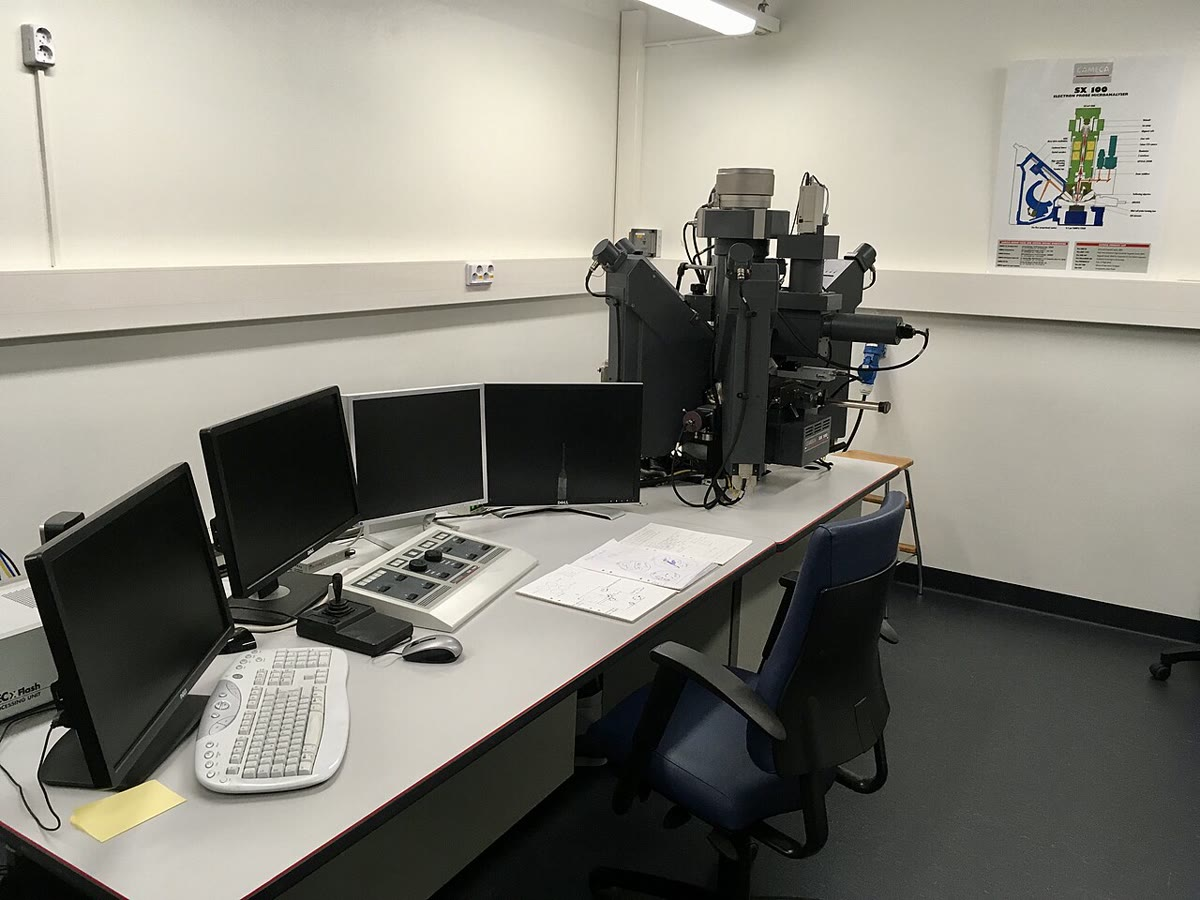
\includegraphics[width=\linewidth]{images/book4/b2-31-microprobe.jpg}
\par\smallskip{\scriptsize \omterm{def:b2:field-lab-methods-2:epma}{电子探针}：电子柱及周围的谱仪，
以及操作员的工作台。照片：Kallerna，CC BY-SA 4.0（维基共享资源）。}
\end{minipage}
\end{inthelab}
% ledger: sercE:epma-spot, sercE:coating, photo:b2-31-microprobe

\section{同位素分析}\label{sec:b2:field-lab-methods-2:isotopes}

\omterm{def:b2:isotope-geochemistry:tracer}{放射成因同位素示踪剂}与年龄（\cref{ch:b2:isotope-geochemistry}）依赖于比值的测定，其精度达
0.01--\qty{0.001}{\percent}；所用元素由岩石经溶解和离子交换色谱法分离，
并在洁净实验室中进行，实验室用的空气经过滤（通常为 100 至
1000 级），以免尘埃给微量样品引入杂质。
% ledger: sercT:tims

\begin{definition}[热电离质谱法，多接收电感耦合等离子体质谱，质量偏倚]\label{def:b2:field-lab-methods-2:tims}
在\emph{热电离质谱法}\index{热电离质谱法}（TIMS）中，
将纯化元素装于薄金属带上，在真空中加热使其电离；离子
在至多 \qty{10}{kV} 的电势差下加速，经磁扇区按质量分离
并收集。在\emph{多接收电感耦合等离子体质谱}\index{多接收电感耦合等离子体质谱}中，离子来自
电感耦合等离子体，它能使难以热电离的元素电离，并且多个
接收器同时测量不同质量的离子束。\emph{质量
偏倚}\index{质量偏倚}是测量值偏离样品真实同位素比值的量，
由仪器引起，即仪器对一种质量的离子
的传输或电离比另一种更容易。
\end{definition}
% ledger: sercT:tims, sercM:mcicpms

两种仪器都能达到此精度。TIMS 通常只电离不到
\qty{1}{\percent} 的原子，其\omterm{def:b2:field-lab-methods-2:tims}{质量偏倚}在一次测定中不断变化。偏倚的校正方法是固定
两种不因衰变而改变的同位素比值，这要求元素至少有三种同位素，其中两种稳定且
非放射成因。对于锶，$^{86}\mathrm{Sr}/^{88}\mathrm{Sr}$ 固定为 0.1194，一种常用的
校正形式是指数律。
% ledger: sercT:tims, sercM:mcicpms, cheong14:mass-bias, ciaaw:sr-isotopes

\begin{proposition}[质量偏倚的指数律]\label{prop:b2:field-lab-methods-2:bias}
假设质量分别为 $m_i$ 与 $m_j$ 的两种同位素的每个测得比值，
与真实比值的关系为 $R_{ij}^{\mathrm{true}} = R_{ij}^{\mathrm{meas}}\,(m_i/m_j)^{\beta}$，整个测定过程中只取一个指数
$\beta$。设参考对的测得比值为 $r$，
其真实值 $r_0$ 已知，则可得
\begin{equation}
\beta = \frac{\ln(r_0/r)}{\ln(m_k/m_l)}
\label{eq:b2:field-lab-methods-2:beta}
\end{equation}
对参考对 $k/l$，而其余各比值均以同一 $\beta$ 进行校正。
\end{proposition}

\begin{proof}
将定律用于参考对，得 $r_0 = r\,(m_k/m_l)^\beta$；两边取对数，
得 $\ln(r_0/r) = \beta\ln(m_k/m_l)$，即 \eqref{eq:b2:field-lab-methods-2:beta}。该指数
由假设对本次测定的各比值都相同，故可校正每一比值。
\end{proof}

锶的参考对为 $^{86}\mathrm{Sr}/^{88}\mathrm{Sr}$，取 $r_0 = 0.1194$，
校正后的 $^{87}\mathrm{Sr}/^{86}\mathrm{Sr}$ 等于测得比值乘以
$(m_{87}/m_{86})^\beta$。按 CIAAW 丰度，锶-86 占 \qty{9.86}{\percent}，
锶-88 占 \qty{82.58}{\percent}，所得结果相同。每次测定还运行\omterm{def:b2:isotope-geochemistry:standards}{同位素参考标准}：
一家实验室对参考物质 NBS~987 进行了七次测定，得 $^{87}\mathrm{Sr}/^{86}\mathrm{Sr} = 0.710252 \pm
0.000007$。
% ledger: cheong14:mass-bias, ciaaw:sr-isotopes

仅凭比值无法得到浓度。为此，取已知量的\emph{稀释剂}，
即某元素经人工富集于某一同位素后的溶液，在化学处理前与溶解的样品混合，
然后测量混合物中的比值。TIMS 实验室用它同时测定
浓度与母子体比值。
% ledger: sercT:tims

\begin{proposition}[同位素稀释]\label{prop:b2:field-lab-methods-2:id}
设样品中含 $N_x$ 摩尔参考同位素 $b$，加入的稀释剂中含 $N_s$ 摩尔该同位素，并设
$R_x$、$R_s$ 与 $R_m$ 分别为另一同位素 $a$ 对 $b$ 在样品、稀释剂和
混合物中的比值。则
\begin{equation}
N_x = N_s\,\frac{R_s - R_m}{R_m - R_x} .
\label{eq:b2:field-lab-methods-2:id}
\end{equation}
相对误差 $\varepsilon$ 作用于 $R_m$，使 $N_x$ 的相对误差为 $\mathcal{M}\varepsilon$，
误差放大因子为
\begin{equation}
\mathcal{M} = \frac{R_m\,(R_s - R_x)}{(R_s - R_m)(R_m - R_x)} ,
\label{eq:b2:field-lab-methods-2:mag}
\end{equation}
当 $R_m = \sqrt{R_s R_x}$ 时最小。
\end{proposition}
\index{同位素稀释}

\begin{proof}
同位素 $a$ 在混合中守恒：$R_m(N_x + N_s) = R_x N_x + R_s N_s$，故 $N_x(R_m - R_x) =
N_s(R_s - R_m)$，即 \eqref{eq:b2:field-lab-methods-2:id}。其对数导数为
$\mathrm{d}\ln N_x/\mathrm{d}\ln R_m = R_m\,[-1/(R_s - R_m) - 1/(R_m - R_x)] = -\mathcal{M}$，其中
$\mathcal{M}$ 如 \eqref{eq:b2:field-lab-methods-2:mag} 所示。在相差正常数 $R_s - R_x$ 的意义下，
$1/\mathcal{M} = (R_s - R_m)(R_m - R_x)/R_m = R_s + R_x - R_m - R_sR_x/R_m$，其导数
$-1 + R_sR_x/R_m^2$ 在 $R_m = \sqrt{R_sR_x}$ 处为零，此时 $1/\mathcal{M}$ 取极大值。
\end{proof}

\omterm{prop:b2:field-lab-methods-2:id}{同位素稀释}既不需要标准曲线，也不要求元素在
化学处理中完全回收：样品与稀释剂一经混合，损失同等作用于两者。
例如，一种已发表的锶稀释剂中，锶-84 占 \qty{99.65}{\percent}，
$^{84}\mathrm{Sr}/^{88}\mathrm{Sr} = 561.4$，$^{86}\mathrm{Sr}/^{88}\mathrm{Sr} = 0.7661$，
每克溶液含锶 \qty{15.271}{\micro\gram}。其 86/88 比值说明，
加入稀释剂后的混合物，其\omterm{def:b2:field-lab-methods-2:tims}{质量偏倚}不能通过将 $^{86}\mathrm{Sr}/^{88}\mathrm{Sr}$ 固定为其
天然值来校正，因为稀释剂已改变了该比值。
% ledger: cheong14:spike, cheong14:mass-bias

\section{瓦尔登内露区的填图作业}\label{sec:b2:field-lab-methods-2:campaign}

在瓦尔登背斜的核部，侵蚀已切穿砂\omterm{def:b2:magma-emplacement:bodies}{岩盖}层，暴露出
基底：被花岗岩侵入的片岩。为实验室供应样品的野外工作，始于
野外。沿内露区由西向东布设两条路线，每隔
\qty{100}{m} 设一站点，每站记录岩石单元，在岩石未风化处采集新鲜样品，
样品以站号编号，需测组构者另取定向样品。本图
显示各站点的岩性：共 30 个站，其中 10 个位于花岗岩上，10 个位于砂\omterm{def:b2:magma-emplacement:bodies}{岩盖}层上，1 个位于片岩上，
1 个位于石灰岩上，8 个位于谷底冲积层上，
那里没有岩石出露。

\begin{omfigure}
\centering
\begin{tikzpicture}
\begin{axis}[axis equal image, xmin=2.4, xmax=4.6, ymin=3.1, ymax=5.0, width=0.66\linewidth,
  tick label style={font=\scriptsize}, xlabel={东向 (km)}, ylabel={北向 (km)},
  label style={font=\small}]
% units: figdata/shared/region.py (read only); stations: figdata/bachelor-2/labmethods.py part stations
\addplot[lith schist, draw=black, line width=0.3pt, even odd rule] table {figdata/out/shared-region-unit-schist.dat};
\addplot[lith granite, draw=black, line width=0.3pt, even odd rule] table {figdata/out/shared-region-unit-granite.dat};
\addplot[om lith={icsTriassic!35}{om sand}, draw=black, line width=0.3pt, even odd rule] table {figdata/out/shared-region-unit-sandstone.dat};
\addplot[om lith={icsJurassic!40}{om limestone}, draw=black, line width=0.3pt, even odd rule] table {figdata/out/shared-region-unit-limestone.dat};
\addplot[om lith={icsJurassic!15}{om shale}, draw=black, line width=0.3pt, even odd rule] table {figdata/out/shared-region-unit-shale.dat};
\addplot[lith alluvium, draw=black, line width=0.3pt, even odd rule] table {figdata/out/shared-region-unit-alluvium.dat};
\addplot[river] table {figdata/out/shared-region-river.dat};
\addplot[only marks, mark=*, mark size=1.6pt, mark options={fill=white, draw=black}]
  table[x=x_km, y=y_km] {figdata/out/bachelor-2-labmethods-stations.dat};
\addplot[only marks, mark=*, mark size=1.6pt, mark options={fill=omThm, draw=black},
  x filter/.expression={\thisrow{unit}==2 ? x : nan}]
  table[x=x_km, y=y_km] {figdata/out/bachelor-2-labmethods-stations.dat};
\node[font=\scriptsize, fill=white, inner sep=1pt, anchor=east] at (axis cs:2.76,3.7) {1};
\node[font=\scriptsize, fill=white, inner sep=1pt, anchor=west] at (axis cs:4.24,3.7) {15};
\node[font=\scriptsize, fill=white, inner sep=1pt, anchor=east] at (axis cs:2.76,4.4) {16};
\node[font=\scriptsize, fill=white, inner sep=1pt, anchor=west] at (axis cs:4.24,4.4) {30};
\draw[black, line width=0.5pt] (axis cs:3.5,4.44) -- (axis cs:3.5,4.62);
\node[font=\scriptsize, fill=white, inner sep=1pt, anchor=south] at (axis cs:3.5,4.62) {第 23 站};
\pic at (axis cs:4.45,4.75) {northarrow};
\end{axis}
\end{tikzpicture}
\par\smallskip{\small 瓦尔登丘陵的基底内露区，图中为两条由西向东路线上的 30 个站点，
相距 \qty{100}{m}。红点：花岗岩上的站点。粉色加叉：花岗岩；灰色：片岩；紫色：三叠纪
砂岩；蓝色：侏罗纪石灰岩；浅蓝色：侏罗纪页岩；奶油色：河流冲积层，河流
向东流。周末问题
的花岗岩样品取自第 23 站。}
\end{omfigure}

\begin{inthefield}[为实验室采样]
\centering
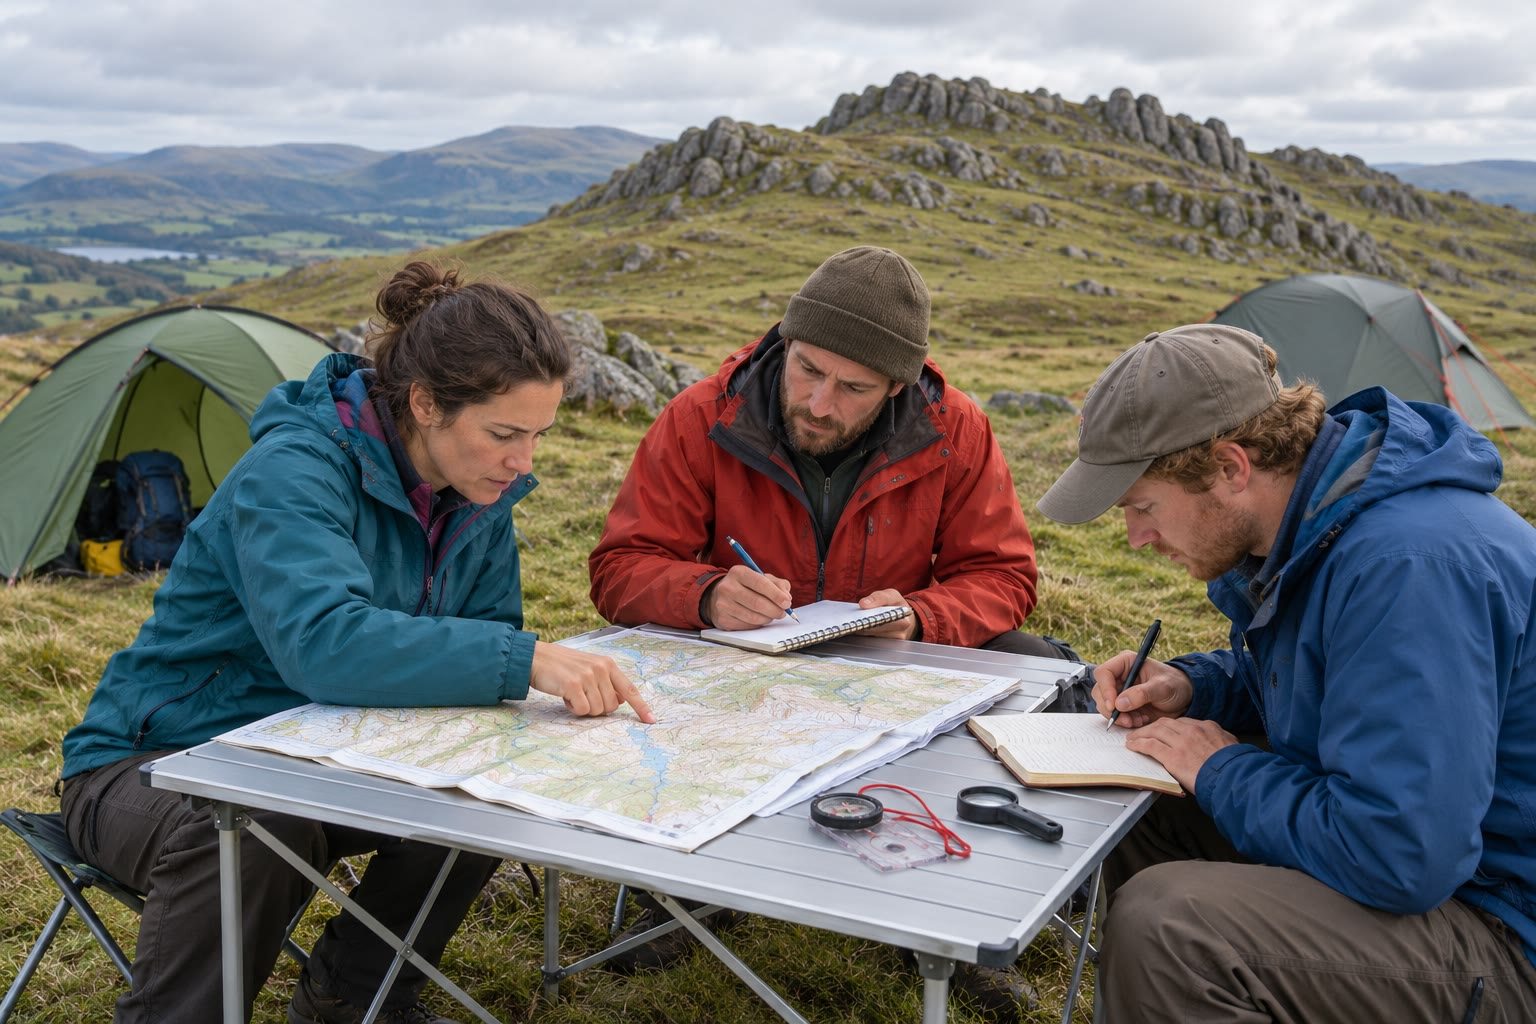
\includegraphics[width=0.56\linewidth]{images/book4/ai/b2-field-camp.jpg}
\par\smallskip{\small 野外小组正在规划次日的路线（AI 生成插图）。}
\par\medskip\raggedright
傍晚，小组将各站点标注到图上，核对记录本中每个样品编号与样品袋
是否一一对应，并确定各样品送往哪个实验室。每个岩石单元取一块
送往薄片实验室；最新鲜的花岗岩与片岩
送去破碎并做全岩分析；另留出少量花岗岩样品供同位素分析。站号
伴随每个样品经历每一步，从样品袋到薄片、
粉末、\omterm{def:b2:field-lab-methods-2:xrf}{熔融玻璃片}，直至数据表中的一行，以便任何异常结果都能追溯到其
露头。
\end{inthefield}

\section{数值的质量}\label{sec:b2:field-lab-methods-2:quality}

每一步都会引入各自的误差，本章的方法涉及化学书中区分的两类误差：
计点法与同位素比值的误差大多是随机的，随计数增加而减小，
其大致按 $1/\sqrt n$ 的规律减小；标定则带有系统误差，
重复测量不能使其减小，只有标准物质才能将其揭示。二氧化硅分析的图同时展示了两者：
柱形长度即方法的精密度；若某数据点偏离零点的量是其柱长除以分析次数平方根的许多倍，
则表明存在偏差。同一元素用两种方法测定，
即用 XRF 与\omterm{prop:b2:field-lab-methods-2:id}{同位素稀释}法测定锶，是进一步的检验，因为两者
不共用任何标定。结果须连同其不确定度一并报告，并按不确定度取位，同时附上同步测定的标准物质数据；
缺少这些数据的数值无法与任何其他数值比较。

\section*{练习}\label{sec:b2:field-lab-methods-2:exercises}

除另有说明外，练习所用数据如下：原子质量 H 1.008、O 15.999、Mg 24.305、Al
26.982、Si 28.085、K 39.098、Sr 87.62；同位素质量 $^{86}\mathrm{Sr}$ 85.909261、
$^{87}\mathrm{Sr}$ 86.908878、$^{88}\mathrm{Sr}$ 87.905612；天然锶中
$^{84}\mathrm{Sr}/^{86}\mathrm{Sr} = 0.05680$，\qty{9.86}{\percent} 为 $^{86}\mathrm{Sr}$ 的丰度；正文中的稀释剂
$^{84}\mathrm{Sr}/^{86}\mathrm{Sr} = 732.8$，\qty{0.13599}{\percent} 为
$^{86}\mathrm{Sr}$ 的丰度，原子量 83.9242，\qty{15.271}{\micro\gram\per\gram}。除另有说明外，
结果取三位有效数字。
% ledger: ciaaw:H, ciaaw:O, ciaaw:Mg, ciaaw:Al, ciaaw:Si, ciaaw:K, ciaaw:sr-isotopes, cheong14:spike

\begin{exercise}[$\star$]\label{exo:b2:field-lab-methods-2:1}
(a) 说出下列结构或晶体的名称：(i) 辉绿岩，其中斜长石板条被完全包裹在
大的普通辉石晶体之中；(ii) 由等大方解石颗粒组成的大理岩，其平直晶界三三相交；
(iii) 云母片岩中一颗长 \qty{5}{mm} 的十字石晶体，内含大量石英包裹体；
(iv) 一颗被连续斜长石与辉石环带包围的石榴子石。(b) 三条晶界相交于
\ang{104}、\ang{128} 和 \ang{128}。求面对 \ang{104} 角的晶界张力与
其余两条晶界张力之比。
\end{exercise}

\begin{exercise}[$\star$]\label{exo:b2:field-lab-methods-2:2}
某粗粒岩石含 \qty{25}{\percent} 石英、15 碱性长石、40 斜长石、12
黑云母和 8 角闪石。(a) 重新计算 Q、A 和 P。(b) 求 P/(A+P)，并命名该岩石。(c) 求
其色指数，并予以定性。
\end{exercise}

\begin{exercise}[$\star$]\label{exo:b2:field-lab-methods-2:3}
某次计数 800 个点，测得某矿物占 \qty{12}{\percent}。(a) 求该比例的
标准差及其相对值。(b) 若改为 3200 个点，结果如何？
\end{exercise}

\begin{exercise}[$\star$]\label{exo:b2:field-lab-methods-2:4}
一份 \qty{0.8000}{g} 的粉末灼烧后质量为 \qty{0.7712}{g}，其残渣与
\qty{8.0000}{g} 助熔剂熔融。(a) 求烧失量。(b) 求样品在熔珠中的质量分数。
(c) 玻璃中 \ce{SiO2} 含量为 \qty{5.20}{\percent}，求灼烧后粉末及原始粉末的
二氧化硅含量。
\end{exercise}

\begin{exercise}[$\star\star$]\label{exo:b2:field-lab-methods-2:5}
(a) 要测定占岩石 \qty{2}{\percent} 的副矿物，使其相对标准误差为
\qty{10}{\percent}，需要计多少个点？(b) 若矿物占 \qty{30}{\percent}，
相对误差相同，又需要多少个点？(c) 评述稀有矿物所需的工作量。
\end{exercise}

\begin{exercise}[$\star\star$]\label{exo:b2:field-lab-methods-2:6}
图中 USGS 的结果显示，流纹岩 RGM-1 测得 \ce{SiO2} $= 72.89$，标准差
为 0.19（20 次分析，推荐值 73.45）；玄武岩 BCR-2 测得 54.17，标准差为 0.13
（20 次分析，推荐值 54.1）。(a) 求各自的回收率，以百分数表示。(b) 求各平均值的
标准差，并以其为单位表示各自与推荐值之差。
(c) 哪一个结果显示存在偏差？对 RGM-1 而言，该方法的精密度是否较低？
\end{exercise}

\begin{exercise}[$\star\star$]\label{exo:b2:field-lab-methods-2:7}
对纯金云母 $\mathrm{KMg_3AlSi_3O_{10}(OH)_2}$ 的\omterm{def:b2:field-lab-methods-2:epma}{电子探针}分析需加以核对。
(a) 求该化学式的摩尔质量，以及其中 \ce{H2O} 的质量分数。(b) 求
\ce{K2O}、\ce{MgO}、\ce{Al2O3} 和 \ce{SiO2} 的质量分数，以及精确分析应得的总量。
(c) 为何云母的总量约为 \qty{96}{\percent} 并非分析不良？
\end{exercise}

\begin{exercise}[$\star\star$]\label{exo:b2:field-lab-methods-2:8}
对锶标准样品进行 TIMS 测定，得 $^{86}\mathrm{Sr}/^{88}\mathrm{Sr} = 0.11905$，且
$^{87}\mathrm{Sr}/^{86}\mathrm{Sr} = 0.71062$。(a) 求指数定律中的指数 $\beta$。
(b) 将 $^{87}\mathrm{Sr}/^{86}\mathrm{Sr}$ 比值校正至小数点后五位。(c) 测定中
本次测定中偏向于轻同位素还是重同位素？
\end{exercise}

\begin{exercise}[$\star\star$]\label{exo:b2:field-lab-methods-2:9}
为检验\omterm{prop:b2:field-lab-methods-2:id}{同位素稀释}法的结果，某实验室向参考玄武岩 BHVO-2 的 \qty{0.0500}{g} 样品中加入
\qty{0.1000}{g} 正文所用的稀释剂，并测得混合物中 $^{84}\mathrm{Sr}/^{86}\mathrm{Sr} =
0.874$。(a) 求所取稀释剂等分试样中 $^{86}\mathrm{Sr}$ 的摩尔数。(b) 求
样品中 $^{86}\mathrm{Sr}$ 的摩尔数，并求其锶浓度（以 ppm 计）。(c) 与推荐值
\qty{394.1}{ppm} 相比较。
\end{exercise}

\begin{exercise}[$\star\star\star$]\label{exo:b2:field-lab-methods-2:10}
对正文所述的锶稀释剂（$R_s = 732.8$，$R_x = 0.05680$）：(a) 求使误差放大因子最小的\omterm{def:b2:atmospheric-thermodynamics:moist-air}{混合比}，
及其在该处的值；(b) 求 $\mathcal M$ 在
$R_m = 0.1$、0.5、1.664 和 100 处的值；(c) 说明
为何应避免混合物接近任一端元，以及分析者在实际中有多大的选择余地。
\end{exercise}

\begin{exercise}[$\star\star\star$]\label{exo:b2:field-lab-methods-2:11}
某花岗岩计数得长石点 400 个，其中 \qty{62}{\percent} 为斜长石。(a) 将长石点中的斜长石
视为二项计数，求 P/(A+P) 的标准差。(b) 该结果距花岗闪长岩边界相差多少个标准差？
(c) 若要使其恰好距边界两个标准差，
需计数多少个长石点？
\end{exercise}

\begin{exercise}[$\star\star\star$]\label{exo:b2:field-lab-methods-2:12}
某矿物占岩石的比例为 $p$。(a) 证明：$n$ 个独立取点均未击中该矿物的概率为
$(1-p)^n$。(b) 若要使至少击中一次占岩石 \qty{1}{\percent} 的矿物的概率不低于 \qty{95}{\percent}，
需要多少个点？(c) 对锆石做同样计算，其占比为
\qty{0.05}{\percent}，并由此说明应如何寻找副矿物。
\end{exercise}

\section*{周末问题}

\begin{problem}[{周末问题——从露头到分析}]\label{pb:b2:field-lab-methods-2:1}
% invented sample; data: ledger rows below; values: calc/ch31.py
瓦尔登花岗岩样品 VH-23 采自本次考察的 23 号站点。取一片薄片，
在规则网格上计点 1200 个：石英 372，碱性长石 348，斜长石 324，
黑云母 108，白云母 36，不透明氧化物 12。取一份 \qty{0.8000}{g} 的粉末，
在 \qty{925}{\celsius} 灼烧后质量为 \qty{0.7949}{g}，随后与 \qty{8.0000}{g} 助熔剂熔融。三种标准物质熔珠给出的
\ce{SiO2} 强度（每秒千次计数，kcps）分别为：BCR-2，
推荐值 \qty{54.1}{\percent}，21.66；AGV-2，59.3，23.70；RGM-1，73.45，29.37；花岗岩熔珠
为 28.63。花岗岩其余氧化物之和为 \qty{27.15}{\percent}。同位素分析方面，
取 \qty{0.1000}{g} 粉末溶解后，与 \qty{0.2500}{g} 正文所述的稀释剂混合；
假定样品具有练习中给出的天然锶丰度。
计算所用数据均取自练习。

\noindent\textbf{第一部分——\omterm{def:b2:field-lab-methods-2:modal}{实际矿物含量分析}。}
\begin{enumerate}
  \item 求各矿物的实际含量比例。
  \item 求石英比例的标准差，以及白云母比例的
        相对标准差。
  \item 求 $M$ 与色指数 $M'$，并给岩石定名。
  \item 将 Q、A、P 重新换算为和为 100。
  \item 求 P/(A+P)，并在 \omterm{def:b2:magmatic-series:qapf}{QAPF 图解}上给岩石定名。
  \item 以 672 个长石点计算 P/(A+P) 的二项标准差，所定名称
        是否可靠？
  \item 要使石英比例的标准差达到一个百分点，需要计数
        多少个点？
\end{enumerate}

\noindent\textbf{第二部分——X 射线荧光法测定二氧化硅。}
\begin{enumerate}[resume]
  \item 求烧失量。
  \item 求样品在熔珠中的质量分数，以及若灼烧后的粉末含
        \qty{72}{\percent}，则玻璃中的二氧化硅。
  \item 通过三种标准物质拟合最小二乘直线 $c = aI + b$，取 $a$ 至
        四位小数，$b$ 至两位小数。
  \item 求花岗岩的 \ce{SiO2}，取两位小数。
  \item 求三种标准物质的残差。该直线是否足够好？
  \item 将各氧化物与烧失量相加。USGS 方法能否重复此分析？
  \item 扣除挥发分后，将二氧化硅重新换算为和为 100。
\end{enumerate}

\noindent\textbf{第三部分——\omterm{def:b2:field-lab-methods-2:tims}{质量偏倚}。}
\begin{enumerate}[resume]
  \item 由 CIAAW 丰度求天然的 $^{86}\mathrm{Sr}/^{88}\mathrm{Sr}$，并与
        用于归一化的值相比较。
  \item 一份未加稀释剂的分样给出 $^{86}\mathrm{Sr}/^{88}\mathrm{Sr} = 0.11853$。求 $\beta$ 至
        四位小数。
  \item 该分样给出 $^{87}\mathrm{Sr}/^{86}\mathrm{Sr} = 0.71655$。对其进行校正，取五位小数。
  \item 求每质量单位的偏倚，以百分数表示。
  \item 为何不能对第四部分的稀释混合物进行此项校正？
\end{enumerate}

\noindent\textbf{第四部分——\omterm{prop:b2:field-lab-methods-2:id}{同位素稀释}法。}
\begin{enumerate}[resume]
  \item 验证稀释剂中含 \qty{99.65}{\percent} 的锶-84 与 \qty{0.13599}{\percent}
        的锶-86。
  \item 求稀释剂分样中锶及 $^{86}\mathrm{Sr}$ 的摩尔数，取四位
        有效数字。
  \item 核对练习中的数值 $R_s = 732.8$ 与 $R_x = 0.05680$。
  \item 混合物校正后的比值为 $R_m = 1.6812$。求样品中 $^{86}\mathrm{Sr}$
        的摩尔数。
  \item 求误差放大因子。若 $R_m$ 已知至 \qty{0.01}{\percent}，稀释剂
        浓度为 $\pm\qty{0.031}{\micro\gram\per\gram}$，求结果的
        相对不确定度。
  \item 求瓦尔登花岗岩中锶的浓度，单位为 ppm。
\end{enumerate}
\end{problem}
% ledger: bgsI:qapf, bgsI:colour-index, usgsT:procedure, usgsT:sio2-table, ciaaw:sr-isotopes, cheong14:spike, cheong14:mass-bias
